\documentclass[conference,9pt,letterpaper]{IEEEtran}
\usepackage[T1]{fontenc}
\usepackage{newtxtext,newtxmath}
\usepackage{graphicx}
\usepackage{booktabs}
\usepackage{amsmath}
\usepackage{array}
\usepackage{xcolor}
\usepackage{soul}
\DeclareRobustCommand{\pending}[1]{{\sethlcolor{yellow}\hl{#1}}}
\setlength{\abovecaptionskip}{3pt}
\setlength{\belowcaptionskip}{2pt}
\setlength{\intextsep}{6pt plus 1pt minus 1pt}
\setlength{\textfloatsep}{7pt plus 1pt minus 1pt}
\setlength{\floatsep}{6pt plus 1pt minus 1pt}
\usepackage{cite}
\usepackage{url}
\usepackage{stfloats}
\usepackage{balance}
\makeatletter
\patchcmd{\@BAlancecol}
 {\setbox\@leftcolumn=\vbox to \@tempdima}
 {\@tempdimb=\ht1\advance\@tempdimb by\dp1
  \ifdim\@tempdimb>\@tempdima\@tempdima=\@tempdimb\fi
  \@tempdimb=\ht3\advance\@tempdimb by\dp3
  \ifdim\@tempdimb>\@tempdima\@tempdima=\@tempdimb\fi
  \setbox\@leftcolumn=\vbox to \@tempdima}
 {\typeout{MECC: balance packing includes split-box depth.}}
 {\errmessage{Failed to patch balanced-column packing}}
\makeatother
\usepackage{capt-of}
\usepackage{float}
\usepackage{needspace}
\setcounter{dbltopnumber}{3}
\renewcommand{\dbltopfraction}{0.85}
\renewcommand{\textfraction}{0.10}
\newcommand{\mecc}{\textsc{MECC}}
\newcommand{\BH}{B_{\mathrm H}}
\newcommand{\BC}{B_{\mathrm C}}
\newcommand{\KH}{K_{\mathrm H}}
\newcommand{\KC}{K_{\mathrm C}}
\newtheorem{proposition}{Proposition}
\title{MECC: Single-GPU MoE Inference with\protect\\Compiler-Guided Three-Tier Expert Caching}
% Anonymous review copy: no author names or affiliation spacer rows.
\author{}
\usepackage[hidelinks]{hyperref}
\hypersetup{pdftitle={MECC: Single-GPU MoE Inference with Compiler-Guided Three-Tier Expert Caching},pdfauthor={}}
\begin{document}
\maketitle\raggedbottom
\begin{abstract}
Single-GPU mixture-of-experts (MoE) inference stores expert weights across memory tiers. Weight delivery introduces HDD reads and host-to-device transfers along the inference path. We present MECC, the MoE Expert Cache Compiler, to coordinate placement and replacement. The compiler allocates per-layer capacity and initializes expert residency from access profiles. The runtime promotes selected experts and retains GPU victims in host memory. Ordered reads and copies deliver weights for GPU execution. On one A100, MECC takes 7.38~s per decode token for FP16 Mixtral-8x7B with uniform initialization. Decode speedups are 1.77$\times$ over streaming and 2.95$\times$ over fixed CPU retention. Perplexity matches these controls.
\end{abstract}

\begin{IEEEkeywords}
Mixture of experts, single-GPU inference, expert offloading, three-tier caching, hardware/software co-design.
\end{IEEEkeywords}

\section{Introduction}
Mixture-of-experts (MoE) models expand parameter capacity through sparse expert activation~\cite{shazeer,switch,mixtral,deepseekmoe}. Each token selects a subset of experts at each MoE layer. Single-GPU deployment places their weights across high-bandwidth memory (HBM), host memory, and a hard disk drive (HDD). This hierarchy combines GPU execution with host caching and backing-store capacity. Expert placement determines the source of each selected weight. An HBM hit supplies the GPU directly. A host hit supplies a host-to-device (H2D) copy. A cold request first reads the expert from HDD. The resulting delivery cost repeats across layers and generated tokens. A prompt first enters prefill, which groups its token rows by selected experts. Decode then revisits the MoE layers for each generated token. Each visit updates the resident expert set. An expert used during prefill can serve later decode requests from memory. Retaining that state across visits avoids repeated delivery. Residency management therefore connects the prompt's initial processing to the subsequent token stream. On shared servers, each serving task receives an expert-cache allocation alongside other jobs and model instances. Planning that allocation and preserving the resulting reuse support deployment with one accelerator. The deployment trades accelerator provisioning against the time spent delivering selected experts.

Expert parallelism distributes weights across several GPUs~\cite{deepspeedmoe,tutel,flashmoedist}. Offloading systems combine weight movement, host execution, and expert caching~\cite{offloading,moeinfinity,fiddler,lightning,promoe}. MoE-CORE combines layer-wise capacity allocation, profile initialization, and online replacement~\cite{core}. SSD-LLaMA coordinates RAM/VRAM retention with storage delivery~\cite{ssdllama}. Edge FlashMoE studies replacement for storage-backed expert access~\cite{flashmoe}. These designs connect sparse routing to the memory hierarchy. MECC studies the connection between an initial layer allocation and later cross-tier reuse. The initial plan covers the first expert requests. Subsequent promotions determine which weights survive GPU turnover. A CPU promotion creates a host position for the displaced GPU expert. That victim has just participated in layer execution. Host admission carries its recent use into the next tier. The admitted victim joins other experts competing for host residency. Its position in this order determines which weight survives the next admission. Preserving that victim converts a later cold request into a host hit. Figure~\ref{fig:intro} illustrates this effect through A100 cache controls. Independent caches take 32.94~s per decode token, compared with 7.38~s for joint retention. Their HDD-demand shares are 47.9\% and 12.5\%. These results motivate carrying the reuse order across the HBM/CPU boundary.

\begin{figure}[H]
\centering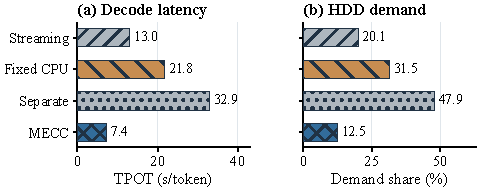
\includegraphics[width=\columnwidth]{measured_figures/intro_evidence.pdf}
\par\nointerlineskip
\caption{Single-A100 expert-cache comparison on Mixtral-8x7B. Joint retention reduces decode time and HDD demand. Separate denotes independent HBM/CPU management.}
\label{fig:intro}
\end{figure}

We present \mecc{}, the MoE Expert Cache Compiler, to connect profile-guided initialization with runtime retention. Compilation ranks experts within each layer and compares the demand covered by another slot. It emits HBM/CPU capacities and the corresponding expert IDs. Each additional slot extends one layer's covered rank. The compiler compares these extensions across layers until it fills the allocation. The emitted IDs then translate that capacity decision into the weight blocks loaded during initialization. Initialization populates those slots from HDD. During inference, the original router supplies selected IDs. An HBM hit updates GPU recency. A CPU hit promotes the selected expert and demotes the HBM victim into the host cache. A cold admission uses the same transition and can replace a host victim. This rule carries recent GPU demand into later host residency. Per-layer capacities stay fixed while membership follows the request stream. The plan preserves layer identity, so equal expert indices in different layers remain separate weight objects. Read and copy ordering then makes the selected weights available to GPU consumers. Prefill batches cold reads across active experts; decode delivers selected experts on demand. Together, compilation, joint retention, and weight delivery connect deployment-time planning to token-by-token execution.

This paper makes three contributions.
\begin{list}{}{\setlength{\leftmargin}{16pt}\setlength{\labelwidth}{14pt}\setlength{\labelsep}{2pt}\setlength{\itemsep}{3pt}\setlength{\topsep}{3pt}}
\item[(1)] \textbf{Profile-guided compilation:} MECC assigns per-layer HBM/CPU slots by marginal covered demand and emits an initial residency plan with expert IDs.
\item[(2)] \textbf{Joint expert retention:} MECC promotes requested experts and preserves GPU victims in host memory. The delivery path orders reads, copies, and GPU consumption.
\item[(3)] \textbf{System evaluation:} we examine decode time, first-token time, source-tier demand, and workload sensitivity. On one A100, MECC takes 7.38~s/token, versus 13.04 for streaming and 21.75 for fixed CPU retention. Component comparisons connect initial placement, victim retention, and transfer exposure to the resulting latency. Deployment comparisons report response time and accelerator occupancy together. Workload plots examine calibration coverage, prompt length, batch size, and profile transfer.
\end{list}
\twocolumn[{
\begin{minipage}{\textwidth}
\centering
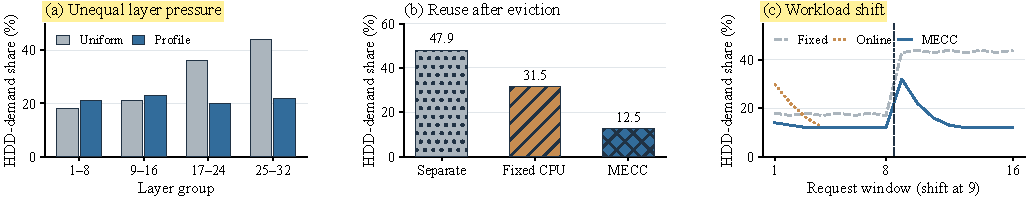
\includegraphics[width=\textwidth]{completion_figures/motivation_evidence.pdf}\par
\vspace{2pt}
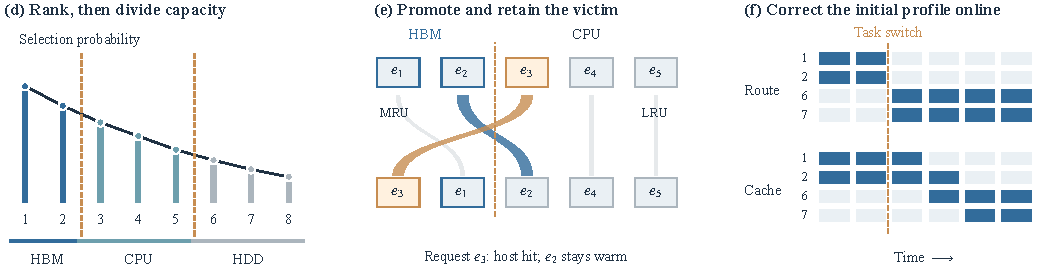
\includegraphics[width=\textwidth]{measured_figures/insights_lower.pdf}
\par\nointerlineskip
\captionof{figure}{Motivation evidence and matching insights. (a--c) compare layer pressure, cross-tier reuse, and workload change; (b) counts A100 demand across all phases. (d--f) show layer-specific capacity cuts, joint victim retention, and online membership updates.}
\label{fig:insights}
\vspace{5pt}
\end{minipage}
}]
\section{Background}
\label{sec:background}
\subsection{Sparse Execution, Full Weight Capacity}
An MoE layer contains a router and a bank of experts. The router selects a small subset for each token, and their weighted outputs form the layer result~\cite{shazeer,switch,gshard}. Mixtral and the DeepSeek family use this separation between active arithmetic and total model capacity~\cite{mixtral,deepseekmoe,deepseekv2,deepseekv3,mixtral22}. Expert identity includes the layer: equal indices in different layers refer to different weights. For input $x$, let $G(x)$ be the selected set and $g_e(x)$ its normalized gate weights. The layer computes
\begin{equation}
y(x)=\sum_{e\in G(x)}g_e(x)E_e(x).
\end{equation}
A generated token passes through successive layers, so expert demand is revealed incrementally during the forward pass. Autoregressive decoding revisits these layers with potentially different selections. Residency changes the location of an immutable expert, while its router score and function remain unchanged.

\subsection{Expert Residency on One GPU}
With enough aggregate HBM, expert parallelism places experts on different GPUs and moves token activations to their owners~\cite{deepspeedmoe,tutel,megablocks,flashmoedist,harmoeny}. A single-GPU deployment instead moves selected weights through the memory hierarchy. Dense layers, activations, and the KV cache compete with experts for HBM; KV management is complementary to expert caching~\cite{pagedattention,sglang}. A CPU hit needs a host-to-device (H2D) copy. An HDD miss first reads the expert into host memory. Heterogeneous inference systems expose these capacity and delivery choices~\cite{flexgen,dsinference,zeroinfinity,llmflash,powerinfer}. We use immutable FP16 experts and retain backing weights on HDD. A resident copy avoids a later cold read, making the history of expert reuse relevant even though routing remains sparse. Prefill groups prompt rows by their selected experts. One fetched expert can serve several rows. Decode advances one token per sequence. These phases expose different amounts of work for hiding delivery.

HBM and CPU retain experts between requests. HDD supplies the complete expert pool. MECC uses the two resident tiers to preserve the weights selected by later tokens.

\section{Motivation and Insights}
\label{sec:challenges}
\subsection{Allocating Slots by Marginal Demand}
A slot can cover different request mass in different layers. Uniform allocation gives each layer the same capacity, even after its hottest experts fit. Figure~\ref{fig:insights}(a,d) connects the resulting pressure to a per-layer capacity cut. The next uncovered expert determines the gain from another slot. Comparing that gain across layers allocates capacity where it covers more demand. Ranking within each layer then determines the initial IDs. Capacity and identity are separate outputs: one sets the room available to a layer, and the other fills it. Routing locality across models has also been studied independently~\cite{routingconsistency}.

\subsection{Preserving Reuse after GPU Eviction}
A GPU eviction changes an expert's location before it determines the expert's next use. If the host retains the weights, another selection avoids HDD. Figure~\ref{fig:insights}(b,e) shows the promotion/demotion decision. Promotion vacates one CPU position as the HBM victim loses its GPU position. Joint retention reuses that host position for the victim. The independent-cache control reports 47.9\% HDD demand, versus 12.5\% for joint retention across all instrumented phases. The cache controls share an initial allocation and expert order. The victim keeps its place in the combined reuse order as it crosses the HBM boundary.

\subsection{Updating Residency beyond Calibration}
A profile summarizes calibration inputs. The next prompt can select a different expert set before a fixed initial placement changes. Figure~\ref{fig:insights}(c,f) pairs the demand shift with an update of resident IDs. The compiler supplies capacities and a starting membership. Recency then changes membership within those capacities. Initial coverage controls early reads; online admission controls the response to later selections. These are separate time intervals in one cache lifecycle. A task switch can expose the distinction even when both methods start with the same profile. Updating IDs from actual requests lets the runtime respond without compiling a new plan or predicting a later gate.

\twocolumn[{
\begin{minipage}{\textwidth}
\section{Overview}
\label{sec:overview}
\centering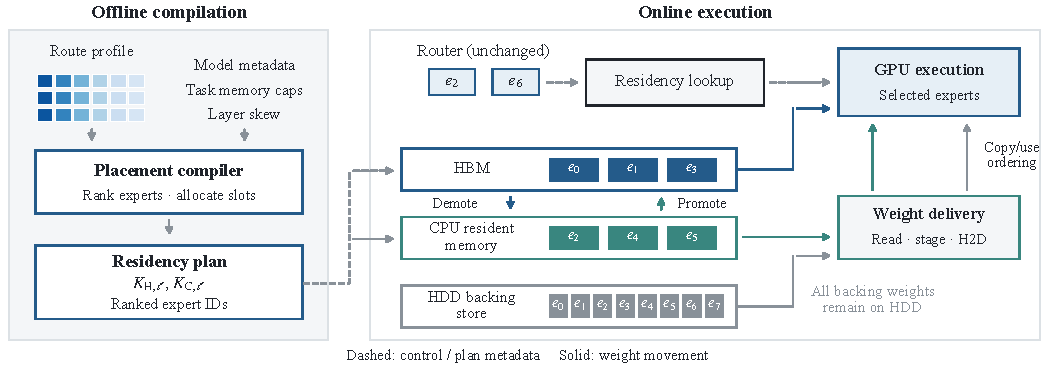
\includegraphics[width=\textwidth]{figures/fig01_overview.pdf}
\par\nointerlineskip
\captionof{figure}{MECC framework. The placement compiler emits per-layer capacities and ranked IDs. Online execution resolves unchanged router selections against HBM, CPU resident memory, and HDD, then delivers weights before their GPU consumers. Dashed arrows carry control or plan metadata; solid arrows move weights.}
\label{fig:overview}

\vspace{8pt}
\end{minipage}
}]

Figure~\ref{fig:overview} follows one model from preparation to inference. Offline profiling supplies layer/expert counts and skew parameters. The compiler combines those inputs with model metadata and task allowances. Its plan records per-layer capacities, ordered IDs, and initial tiers. Initialization reads the specified experts from HDD and populates HBM and CPU. The backing store retains the complete pool.

At each MoE layer, the gate produces selected IDs and weights. Residency lookup chooses HBM, CPU, or HDD as the source. Promotion makes the requested expert available on the GPU. Demotion preserves an HBM victim on the host when the retention rule admits it. Read and copy dependencies then order execution before output aggregation. Each generated token repeats this layer sequence; later tokens reuse the resulting resident state.

The plan, cache state, and delivery path operate at three time scales. The plan fixes per-layer capacities. Accesses change membership and recency. Delivery controls when weights can be consumed. Placement comparisons therefore hold the runtime rule fixed. Retention comparisons hold initial capacities and IDs fixed. Scheduling comparisons use the same demand and resident state. This decomposition links each system decision to its component comparison in Section~\ref{sec:evaluation}.

\section{Method}
\label{sec:method}
\subsection{Compiling Capacities and Initial Identities}
\begin{figure}[H]
\centering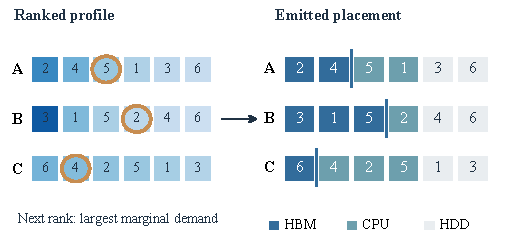
\includegraphics[width=\columnwidth]{method_redesign/compile_frontiers.pdf}
\par\nointerlineskip
\caption{Compiling the initial state. The left grid contains ranked per-layer demand; circles mark the next uncovered candidates. Shared HBM/CPU slot allowances produce different cuts in the emitted rows. A, B, and C identify different layers. }
\label{fig:compile}
\end{figure}

Consider $L$ MoE layers with $N_\ell$ experts per layer. Each model uses equal-size experts and equal top-$k$ across layers. Let $s$ be expert size and let $B_{\mathrm H},B_{\mathrm C}$ be logical expert allowances. They supply $S_{\mathrm H}=\lfloor B_{\mathrm H}/s\rfloor$ HBM slots and $S_{\mathrm C}=\lfloor B_{\mathrm C}/s\rfloor$ CPU slots. Expert slots define the primary residency plan.

The compiler takes an expert order and a skew parameter $\alpha_\ell$ for each layer. Profile counts determine expert order; a discrete Zipf model supplies the marginal slot score:
\begin{equation}
q_{\ell,r}=\frac{r^{-\alpha_\ell}}{\sum_{j=1}^{N_\ell}j^{-\alpha_\ell}},
\qquad p_{\ell,r}=q_{\ell,r}/L.
\end{equation}
Here $r$ denotes an expert rank within layer $\ell$. Equal top-$k$ gives equal layer selection mass. Sorting counts preserves the mapping from each rank to its original expert ID.

Figure~\ref{fig:compile} shows the resulting cuts. A valid plan obeys $\sum_\ell K_{\mathrm H,\ell}\le S_{\mathrm H}$, $\sum_\ell K_{\mathrm C,\ell}\le S_{\mathrm C}$, and $K_{\mathrm H,\ell}+K_{\mathrm C,\ell}\le N_\ell$. The adaptive scan starts with one slot per layer in each fast tier. The remaining capacity supplies ranks beyond these initial slots.

The scan first assigns HBM slots. At each step, it chooses the layer with the largest next-rank score:
\begin{equation}
\Delta_\ell=q_{\ell,K_{\mathrm H,\ell}+1}.
\end{equation}
CPU allocation then compares ranks after each HBM cut. Allocating a slot exposes the next rank in that layer. Layer ID breaks score ties; expert ID breaks count ties. A direct scan costs $O(L(S_{\mathrm H}+S_{\mathrm C}))$ after sorting. The allocation criterion is the demand covered by the next resident expert.

The plan emits per-layer capacities and ordered IDs. Initialization places the first HBM ranks on the GPU and the next CPU ranks on the host. Missing count data selects natural ID order. Capacities stay fixed during a run. Router requests can replace initial residents, including experts absent from the profile.

\subsection{Retaining Victims across the Tier Boundary}
Each layer keeps two ordered resident sets. Most-recently used (MRU) entries precede least-recently used (LRU) entries. HBM holds the first part of the logical order; CPU holds the next part. An HBM hit moves its expert to HBM MRU. A CPU hit removes its host entry and promotes it to HBM MRU. If HBM is full, its LRU victim becomes CPU MRU. CPU pressure removes the CPU LRU. HDD retains every backing expert.

\begin{figure}[H]
\centering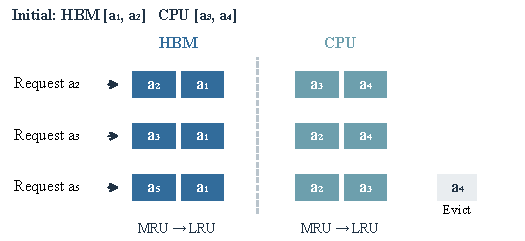
\includegraphics[width=\columnwidth]{method_redesign/residency_cases.pdf}
\par\nointerlineskip
\caption{Three requests from the same initial state. A hit changes recency; a host promotion also demotes the GPU victim; a cold admission can additionally evict the CPU victim. Rows show completed logical states, each ordered MRU to LRU.}
\label{fig:retention}
\end{figure}
Figure~\ref{fig:retention} starts each row from HBM $[a_1,a_2]$ and CPU $[a_3,a_4]$. Requesting $a_2$ changes only HBM recency. Requesting $a_3$ gives HBM $[a_3,a_1]$ and CPU $[a_2,a_4]$. Requesting cold $a_5$ gives HBM $[a_5,a_1]$ and CPU $[a_2,a_3]$; $a_4$ leaves the fast tiers. Promotion preserves the more recent GPU victim in the position vacated on the host.

These completed serial transitions implement exclusive LRU across the combined logical capacity. Batch preparation can promote several experts before their consumers run. The serial stack describes replacement, while the batch path also needs temporary copies and a consumption order. Admission follows current requests while the initial plan supplies the starting order.

The implementation retains a host mirror with each GPU resident. Demotion can reuse that mirror without D2H. The host mirror supplies the weights for demotion. Cache eviction updates membership, while stream tracking preserves storage through GPU consumption.

\subsection{Ordering Delivery before Expert Consumption}
Prefill identifies the experts selected across its token rows. The runtime submits cold reads for those experts and resolves each read at consumption. Figure~\ref{fig:delivery} shows a prefill schedule in which a resident expert executes while another read progresses. Decode delivers selected experts on demand. Both paths consume the original gate output and preserve expert aggregation order.

\begin{figure}[H]
\centering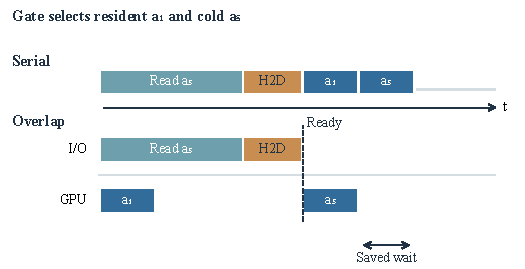
\includegraphics[width=\columnwidth]{method_redesign/delivery_overlap.pdf}
\par\nointerlineskip
\caption{Prefill delivery of resident $a_1$ and cold $a_5$ selected by one gate. Overlap executes ready work during the same read/copy path. The copy/use boundary orders $a_5$'s consumer; the host source remains live through copy completion. }
\label{fig:delivery}
\end{figure}
Completion of a read future makes its host weights available for copying. The implementation then waits on the copy stream before yielding CUDA weights to a consumer. Recording the consuming stream prevents allocator reuse while kernels still reference the tensors. These operations enforce read, copy, and use dependencies. Copy-stream synchronization orders weight availability before GPU execution.

Resident work overlaps the submitted read batch during prefill. Transfer completion advances the next selected expert to GPU consumption. The schedule shortens exposed delivery while preserving the selected expert set. Cache coverage reduces the number of deliveries; overlap reduces the time exposed by each delivery.

\subsection{Sharing the Expert Execution Interface}
Policies share the FP16 loader, model graph, and router. The loader resolves each layer/expert ID to its weight tensors. The router produces the selected set and aggregation weights. The cache chooses the source tier, and delivery prepares the tensors for the same GPU consumer. This interface keeps expert execution aligned across the component comparisons.

\section{Evaluation}
\label{sec:evaluation}
\subsection{Evaluation Overview}
We evaluate expert residency through latency, source-tier demand, and workload sensitivity. Component comparisons separate placement, retention, and delivery. Deployment comparisons connect one-GPU execution to resident accelerator configurations. Appendix~\ref{app:setup} provides configurations, policy definitions, and figure data annotations.

\subsection{Single-GPU Performance}
\begin{figure}[H]
\centering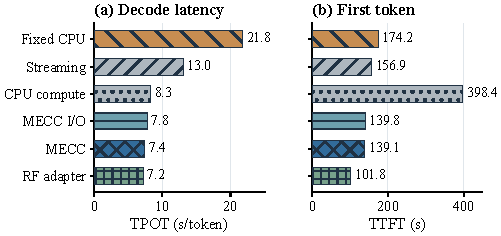
\includegraphics[width=\columnwidth]{measured_figures/main.pdf}
\par\nointerlineskip
\caption{Single-A100 runtime comparison. The panels report per-token decode time and time to first token.}
\label{fig:performance}
\end{figure}
Figure~\ref{fig:performance} reports MECC at 7.38~s/token, streaming at 13.04, and fixed CPU at 21.75: TPOT ratios of 1.77$\times$ and 2.95$\times$. The RF adapter takes 7.19~s, MECC I/O 7.78, and CPU compute 8.26. MECC's TTFT is 139.1~s, versus 156.9 for streaming and 174.2 for fixed CPU. MECC, streaming, fixed CPU, RF, and MECC I/O report PPL 3.427; CPU compute reports 3.432. The two timing panels describe first-token and subsequent-token execution. Expert residency carries weights from prefill into decoding and from one generated token to the next. The retained state supplies later requests from HBM or CPU. The RF and MECC variants explore different host victim choices within this execution path. The I/O variant changes weight delivery while retaining the same demand-driven computation. These comparisons connect latency to residency and scheduling decisions through a shared model interface.

MECC's reported access mix is 77.5\% HBM, 10.0\% CPU, and 12.5\% HDD. RF reports 52.2\% HBM, 36.6\% CPU, and 11.1\% HDD. These distributions show two uses of the fast tiers. MECC has a larger HBM-hit component; RF has a larger host-hit component. GPU hits reuse weights in place. Host hits reuse weights after H2D. The computation consumes the same FP16 experts through these source-specific paths. The residency classifications and timing panels describe lookup outcomes and request latency.

\subsection{Mechanism Attribution}
\label{sec:mechanisms}
\begin{figure*}[!t]
\centering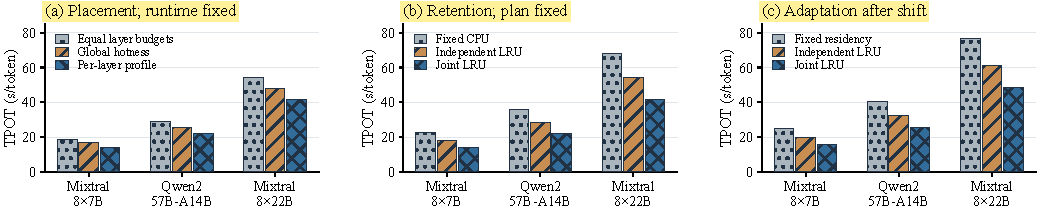
\includegraphics[width=\textwidth]{completion_figures/mechanism_sweeps.pdf}
\par\nointerlineskip
\caption{Component comparisons on three models. (a) Placement with runtime fixed. (b) Retention with initialization fixed. (c) Adaptation after a task switch. The controls isolate initialization, victim retention, and online adaptation, respectively.}
\label{fig:target_mechanisms}
\end{figure*}
Figure~\ref{fig:target_mechanisms} separates placement, retention, and adaptation. For Mixtral-8x7B, the placement comparison moves from \pending{18.6 to 14.2 s/token}, joint retention from \pending{18.3 to 14.2}, and post-switch adaptation from \pending{25.1 to 16.0} relative to fixed residency. The three controls hold runtime, initial plan, and switch protocol fixed, respectively. This separates better initial coverage from preservation of later reuse.

\begin{figure}[H]
\centering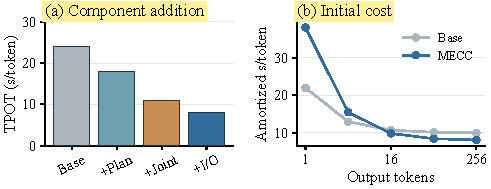
\includegraphics[width=\columnwidth]{completion_figures/ablation_startup.pdf}
\par\nointerlineskip
\caption{Ablation and startup. The right panel reports initialization cost per output token plus decode cost.}
\label{fig:target_ablation}
\end{figure}
Figure~\ref{fig:target_ablation}(a) compares component addition. Its TPOT sequence is \pending{24, 18, 11, and 8 s/token}. The last I/O step retains a \pending{20-percent HDD-demand share}, separating delivery scheduling from miss reduction. Panel (b) uses $T_{\mathrm{avg}}(n)=T_{\mathrm{init}}/n+T_{\mathrm{decode}}$ for $n$ output tokens. The curves cross at \pending{9 output tokens}. Before that point, MECC's initial cost dominates. Later outputs amortize initialization and expose the difference in decode time.

\begin{figure}[H]
\centering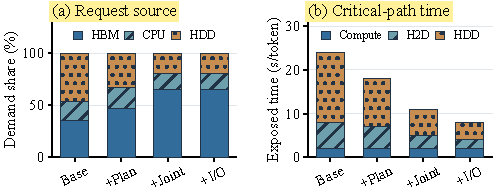
\includegraphics[width=\columnwidth]{completion_figures/traffic_exposure.pdf}
\par\nointerlineskip
\caption{Source demand and exposed time. The last I/O step preserves the demand fractions while shortening the exposed read/copy path.}
\label{fig:target_traffic}
\end{figure}
Figure~\ref{fig:target_traffic} separates cache coverage from scheduling. The HDD share falls from \pending{46 to 20 percent} before the I/O step. Overlap then shortens exposed delivery without changing the resident-set result. The stacked latency components sum to the TPOT values in Figure~\ref{fig:target_ablation}. A source-demand share counts expert requests, while an exposed-time component counts delay on the execution path. A host hit supplies an H2D transfer. A cold request adds a read that can overlap ready GPU work. Keeping both views separates cache coverage from delivery timing. In the source panel, placement and joint retention expand the HBM portion and reduce the HDD portion. In the time panel, those changes reduce exposed read time. The final I/O step retains the source distribution and shortens the transfer components. The two views therefore describe successive effects within the same component sequence: choosing the source of a request, then scheduling its delivery. This interpretation follows the compiler, cache, and delivery stages of the framework.

\subsection{Model and Deployment Scaling}
\begin{figure}[H]
\centering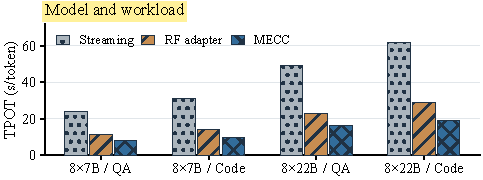
\includegraphics[width=\columnwidth]{completion_figures/cross_model.pdf}
\par\nointerlineskip
\caption{Model and workload comparison. Mixtral-8x7B and 8x22B with QA/code inputs. Each policy uses the same model and workload within a group. }
\label{fig:target_models}
\end{figure}
Figure~\ref{fig:target_models} compares model size and workload. The plotted MECC values range from \pending{8 to 19 s/token}, versus \pending{24 to 62} for streaming and \pending{11 to 29} for the RF adapter. QA and code exercise different expert-demand patterns; increasing model size also changes the expert pool and transfer size. The comparison therefore pairs every policy within each model/workload point.

\begin{figure}[H]
\centering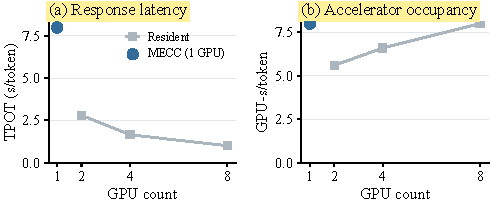
\includegraphics[width=\columnwidth]{completion_figures/gpu_tradeoff.pdf}
\par\nointerlineskip
\caption{One-GPU/resident-reference tradeoff. The panels compare single-GPU MECC with resident configurations and report latency alongside GPU occupancy.}
\label{fig:target_gpu}
\end{figure}
Figure~\ref{fig:target_gpu} separates GPU provisioning from response latency. The endpoint comparison pairs \pending{one GPU at 8 s/token versus eight GPUs at 1 s/token}; both correspond to \pending{8 GPU-s/token}. The \pending{two-GPU resident point uses 5.6 GPU-s/token}, which places the intermediate resident configuration between the endpoint cases. The two panels show the provisioning and response-time tradeoff.

\begin{figure*}[!t]
\centering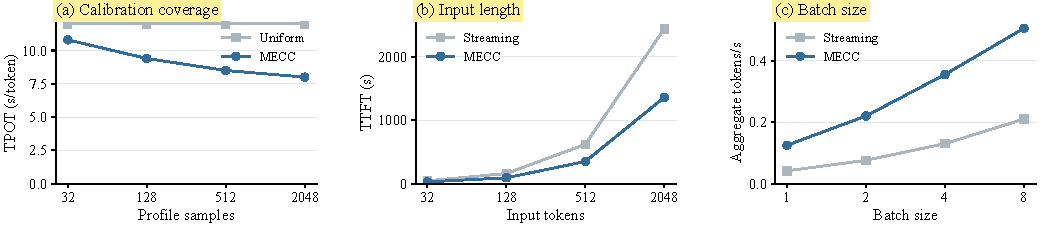
\includegraphics[width=\textwidth]{completion_figures/workload_sensitivity.pdf}
\par\nointerlineskip
\caption{Profile, input-length, and batch sensitivity. Profile size changes initialization quality, input length changes first-token work, and batch size changes aggregate throughput. The panels vary one workload parameter at a time.}
\label{fig:target_sensitivity}
\end{figure*}
\subsection{Capacity and Workload Sensitivity}

The measured 30/60~GB settings give MECC TPOTs of 14.46 and 0.76~s/token, with 32.2\% and zero HDD demand. Four HBM plus four host slots at 60~GB cover all eight experts per layer; zero cold demand is a capacity transition. RF takes 13.06 and 0.74~s/token. The capacity transition replaces HDD delivery with host-to-device transfer.

\begin{figure}[H]
\centering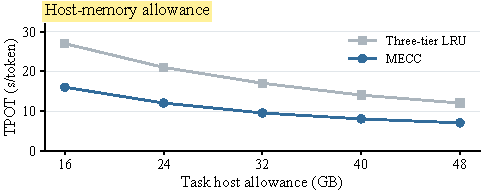
\includegraphics[width=\columnwidth]{completion_figures/quota_targets.pdf}
\par\nointerlineskip
\caption{Host-memory allowance sweep. Five host allowances compare MECC and three-tier LRU within one comparison protocol.}
\label{fig:target_quota}
\end{figure}
Figure~\ref{fig:target_quota} resolves intermediate capacity points. The MECC curve changes from \pending{16 to 7 s/token} over \pending{16--48 GB}, compared with \pending{27 to 12} for three-tier LRU. The sweep separates pressure within the cold-tier regime from the full-coverage threshold. Additional host capacity can first preserve more reused victims, then eliminate cold demand once the complete expert set fits. The latter transition changes the dominant delivery path from HDD plus H2D to H2D alone. The curves connect the allocated host capacity to the delivery path used by later requests.

\begin{figure}[H]
\centering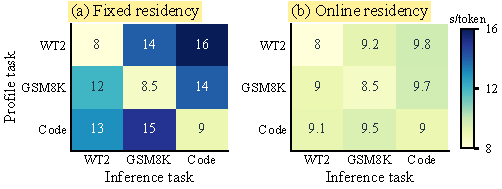
\includegraphics[width=\columnwidth]{completion_figures/profile_mismatch.pdf}
\par\nointerlineskip
\caption{Profile transfer across tasks. Rows select the calibration task and columns the inference task. Cells are TPOT in s/token; the two panels share a color scale.}
\label{fig:target_mismatch}
\end{figure}
Figure~\ref{fig:target_sensitivity} examines scale within a workload. Figure~\ref{fig:target_mismatch} examines transfer between WikiText-2, GSM8K, and code inputs. The off-diagonal cells show profile transfer between tasks. Online membership updates reduce this penalty and preserve the matched-profile behavior.

\balance
\section{Related Work}
\textbf{Layer planning and online residency.} MoE-CORE combines nonuniform device capacity, domain-informed initialization, routing-history-aware replacement, and cross-layer prefetching~\cite{core}. Its main path executes the router-selected experts; substitution is optional. MECC also separates initialization from online membership. Its focus is the connection between per-layer allocation and joint HBM/CPU retention when a selected expert can miss both tiers. MECC connects a compiled layer allocation to the promotion and victim-demotion path across HBM and CPU.

\textbf{Storage-backed expert delivery.} SSD-LLaMA manages bounded RAM and VRAM caches, retains GPU victims on the host when possible, and pipelines expert reads and transfers~\cite{ssdllama}. It also studies lossless transport compression and CPU/GPU execution partitioning. Edge FlashMoE studies device-cache replacement with on-demand storage access~\cite{flashmoe}. MECC keeps FP16 representation and GPU expert execution fixed in its retention controls. Its retention controls use a shared weight format and delivery stack.

\textbf{Offloading, prediction, and execution.} Early expert offloading and SwapMoE expose placement and paging choices~\cite{offloading,swapmoe}. Fiddler and DAOP choose CPU/GPU work; MoE-Lightning pipelines heterogeneous execution; MoE-Infinity uses activation traces~\cite{fiddler,daop,lightning,moeinfinity}. ProMoE, Pre-gated MoE, Fate, and ExpertFlow use proactive caching, lookahead, or token scheduling~\cite{promoe,pregated,fate,expertflow}. HOBBIT and Specter vary loading precision; MoEpic uses segments; SliceMoE uses precision slices; Mira combines staging and quantization~\cite{hobbit,specter,moepic,slicemoe,mira}. ZipMoE uses compression and affinity scheduling~\cite{zipmoe}. These mechanisms change demand prediction, bytes per request, or where computation runs. A comparison of whole-expert retention keeps those choices fixed.

Klotski and Bevy expose work across batches or requests~\cite{klotski,bevy}. OD-MoE distributes on-demand loading across edge nodes; HeteGen studies heterogeneous dense inference~\cite{odmoe,hetegen}. Their scheduling scopes differ from delivery within the current MoE gate. Ready work from another request can hide a wait even when the ongoing request has no resident expert to execute. This distinction separates throughput from the response time of one request.

\section{Conclusion}
\looseness=1
MECC uses an offline plan to initialize a per-layer HBM/CPU expert cache. Online promotion preserves GPU victims on the host as routing changes. The implementation separates replacement from storage lifetime and orders reads and copies before execution. The A100 study reports decode latency, source-tier demand, and sample perplexity under a shared FP16 harness. Placement, retention, and delivery controls expose the decisions behind those outcomes.

\clearpage
\nobalance
\IEEEtriggeratref{24}
\bibliographystyle{IEEEtran}
\bibliography{references}
\clearpage
\appendices
\balance
\section{Experimental Configuration and Figure Data}
\label{app:setup}
\subsection{Hardware and Weight Representation}
The measured testbed uses one NVIDIA A100 80~GB PCIe. Expert weights use FP16. Dense layers and the router execute on the GPU. The expert store resides on a RAID logical volume reporting rotational media through ROTA=1. The manuscript calls this backing tier HDD. The logical-device record identifies the exposed storage path; the controller's physical-drive inventory is a separate platform record.

Each stored expert contains its gate, up, and down weight tensors. Layer and expert IDs identify the block used by the loader. HBM holds GPU residents. Host memory holds CPU residents, mirrors, and staging tensors. HDD retains the complete expert pool throughout inference.

\subsection{Measured Protocols}
The main comparison uses Mixtral-8x7B-Instruct-v0.1, four HBM slots and three CPU slots per layer, and uniform initialization. It processes eight WikiText-2 prompts with 64 input tokens and 64 output tokens. Each policy has one measured run. The planner settings are 50~GB for HBM expert slots and 40~GB for CPU expert slots. Perplexity uses a 1024-token WikiText-2 sample. The same loader and model graph serve the policy comparisons.

The 30/60~GB host-allocation comparison uses four WikiText-2 prompts and 16 output tokens. Its HBM allocation has four slots per layer. At the 60~GB setting, four HBM and four CPU slots cover the eight experts in each layer. The paper presents these points as a separate capacity comparison. The shorter protocol is retained with the corresponding numbers.

\subsection{Policy Definitions}
Streaming loads selected experts through the shared delivery path. Fixed CPU keeps an initial host set and uses GPU replacement. Independent caching updates HBM and CPU recency separately. MECC couples GPU promotion to host admission of the GPU victim. These controls share the model and expert store.

The RF adapter derives its public recency and frequency features from edge FlashMoE. It uses HBM LRU and a CPU score that combines inverse recency with normalized access count. Equal deterministic weights combine the two score terms. The paper labels it RF adapter to identify this mechanism implementation. CPU-compute evaluates selected expert work on the host. The I/O variant supplies a separate delivery control.

For candidate expert $e$, the RF score is $0.5/d_e+0.5f_e/f_{\max}$. Here $d_e$ is recency distance, $f_e$ is cumulative access count, and $f_{\max}$ normalizes frequency. The host cache removes the candidate with the lowest score. Expert ID breaks score ties. The access clock advances on each request.

\subsection{Timing and Demand Counters}
TTFT denotes time to first token. TPOT denotes time per output token during decode. Accelerator occupancy is GPU count multiplied by TPOT, reported in GPU-s/token. It describes accelerator provisioning over response time. The paper reports that product alongside latency.

The measured HDD-demand shares aggregate all instrumented phases. They count classified expert accesses. An expert installed by prefetch is classified by its resident tier at consumption. Read and copy traffic use different byte counters. Initialization, warmup, prefill, decode, and PPL are distinct execution windows. The reported demand percentages retain the aggregate window used by the source runs. The short-window correctness diagnostic compares the streaming and MECC paths through routing, logits, gates, and generated tokens. The reported PPL values use the stated WikiText-2 sample.

\subsection{Figure Data Annotations}
Yellow-highlighted numerical values and panel titles identify authored design targets. They are unmeasured values used to specify the illustrated comparisons. The unhighlighted A100 results come from committed run records. Thus the source of a panel remains distinct from the mechanism illustrated beside it.

The Introduction comparison and single-A100 runtime figure use measured results. In the Motivation figure, panel (b) uses measured aggregate demand; panels (a,c) use design arrays. Panels (d--f), the framework, and the method diagrams describe mechanisms. Their expert IDs, slot counts, and schedules serve as examples of the corresponding operations.

The component, startup, traffic/exposure, cross-model, GPU-occupancy, quota, workload-sensitivity, and profile-transfer plots use design targets. The model labels name the configurations to compare. QA and Code identify the workload groups in those arrays. WikiText-2 and GSM8K identify language-modeling and arithmetic inputs. The Code label identifies the code-input group. These arrays do not add measured model or benchmark runs.

The plotted startup example uses $T_{\mathrm{avg}}(n)=T_{\mathrm{init}}/n+T_{\mathrm{decode}}$. Its crossing at nine output tokens follows from the supplied initial and decode costs. The source-demand stacks sum to 100\%. The exposed-time stacks sum to the component TPOT values. These checks align the panels within the design example.

\subsection{Memory and Execution Accounting}
Planner allowances count primary expert slots. The implementation also retains host mirrors for GPU residents. Those mirrors consume host storage and supply later demotions. Staging and temporary copies add allocations during delivery. Physical accounting therefore tracks primary residency, mirrors, and staging separately from the slot plan.

The compiler library accepts per-layer skew parameters and ranked IDs. The measured main run uses uniform initialization. The non-uniform e2e CLI branch generates layer skew parameters; a calibrated profile is an explicit compiler input. Prefill submits read futures for the selected expert batch. Decode loads experts on demand. Copy-stream synchronization orders CUDA weight consumption, and consuming-stream tracking preserves tensor storage through kernel execution.

\subsection{Plan and Request Records}
A compiled plan stores the model identifier, layer count, experts per layer, expert size, per-layer capacities, and ranked IDs. The capacity arrays define the HBM and CPU cuts. The placement array maps ranks back to original expert identities. Cache initialization consumes both arrays.

\subsection{Source Records}
Committed per-run JSON files supply the A100 measurements. The measured-figure audit lists the run IDs and field mappings. The two design-array files supply the highlighted figures. Their source manifest records field names and SHA-256 hashes. The revision preserves those arrays and the measured plots. Each archived manuscript version includes its sources and an artifact hash record.

\end{document}
